%\documentclass[preprintnumbers,amsmath,amssymb,superscriptaddress,twocolumn,showpacs]{revtex4}
\documentclass[preprintnumbers,amsmath,amssymb]{revtex4}
\usepackage{graphicx}% Include figure files
\usepackage{dcolumn}% Align table columns on decimal point
\usepackage{bm}% bold math
%\usepackage{natbib}
\usepackage{physics}
\usepackage[caption=false]{subfig}

%\newcommand{|}{Y$_2$SiO$_5$}
\def\sgn{\mathop{\rm sgn}}
\newcommand{\be}{\begin{equation}}
\newcommand{\ee}{\end{equation}}

\newcommand{\bea}{\begin{eqnarray}}
\newcommand{\eea}{\end{eqnarray}}


\begin{document}

\title{Cooling the motion of a trapped diamond via NV cross-relaxation}

\maketitle

\tableofcontents

\section{Librational mode susceptibility}

TODO : Inclure couplage au cm. Décrire Sx et Sz comme le fait Arcizet (couplage dispersif et couplage résonnant...)

The equation of motion for the librational mode $\theta(t)$ is 

\begin{eqnarray}I \ddot \theta&=& -I \omega_\theta^2 \theta -I\gamma \dot \theta+\Gamma_{\rm spin}+\Gamma_T,
\end{eqnarray}\label{eqnmotion}
where $I$ is the moment of inertia, $\omega_\theta$ is the angular frequency for that mode. $\gamma$ is the damping rate due to collisions with the background gaz and $\Gamma_T(t)$ is the associated Langevin torque.
$\Gamma_{\rm spin}(\theta)$ is a torque that depends on the angle $\theta$. Fourier Transforming this equation and writing each quantity as $f(\omega)=\langle f \rangle+\delta f (\omega)$ yields to first order 
$$\delta \theta(\omega)=\chi_{\rm eff}(\omega)\delta\Gamma_T(\omega)$$
where
\bea
\chi_{\rm eff}(\omega)&=&\frac{1}{I(\omega_\theta^2-\omega^2-i\omega \gamma)-K(\omega)} \quad {\rm and }\quad K(\omega)=\frac{K_s}{1+i\omega\tau}\\
\eea
Here $K(\omega)$ is a dynamical spin-stiffness. 
It was found by linearizing $\Gamma_{\rm spin}(\omega,\theta)$ about an angle $\theta_0$, yielding $\Gamma_{\rm spin}(\omega,\theta)=\Gamma_{\rm spin}(\theta_0)+K(\omega) (\theta-\theta_0)$. Such a dynamical spring effect arises in the presence of a back action from the mechanical oscillator onto the spins. Note that $K_s$ can either be positive (binding) or negative (anti-binding).
We can rewrite the susceptibility in a condensed form 
\bea
\chi_{\rm eff}(\omega)&=&\frac{1}{I(\tilde\omega_\theta^2-\omega^2-i\omega \tilde\gamma)}
\eea
with 
\bea
\tilde\omega_\theta^2=\omega_\theta^2\big[1+\frac{K_s}{K_t}\frac{1}{1+(\omega_\theta\tau)^2}\big] \quad {\rm and} \quad \tilde\gamma=\gamma\big[1-Q\frac{K_s}{K_t}\frac{\omega_\theta\tau}{1+(\omega_\theta\tau)^2}\big]
\eea
the modified damping a frequencies of the mechanical oscillator.
Here $K_s=I\omega_\theta^2$ is the trap stiffness and $Q=\omega_\theta/\gamma$ is the trap quality factor. A strong delay $\tau$ compared to the trap period $2\pi/\omega_\theta$ enables cooling or heating if $K_s$ is positive/negative.

In practice, there are several ways to achieve such a dynamical stiffness. Photothermal, spin polarisation delay (our nature), ...
Another way induce dynamical backaction : cross-relaxation from two-coupled NV centers. 

We need a torque $\Gamma_{\rm spin}(\theta)$ that varies on a small angular scale to induce a strong restoring force $K$. 
Let us first discuss how to attain a static torque and then how it can be modified using cross-relaxation. 

\section{Static torque}

The static torque is provided by NV centers in the presence of an off-axis magnetic field. 
Physical picture:  Under spin polarisation in the ground state, an off-axis magnetic field tilts the spins away from $z$ (where the spin-spin interaction is minimized) : a torque is then applied to the levitation object to align
back the two spins of the NV spin one triplet to the magnetic field.
Let us calculate the torque from a single NV first.  We will then estimate the total static torque from the four NV centers close to a degeneracy (where cross-relaxation leads to a modified stiffness).

\subsection{Static torque from a single NV}

The hamiltonian of a single NV under a magnetic field is 
\be
\hat{H}=\hbar D S_z^2+\hbar \gamma_e\bm S \cdot \bm B
\ee
We simplify the problem by assuming that the motion is in the $x-z$ plane and that $\gamma_e B \ll D$.
The torque operator 
\be
\hat \tau = -\partial \hat{H} /\partial \theta = \hbar \gamma_e B (\sin\theta \hat{S_x}-\cos\theta \hat{S_z}).
\ee
The mean value of the torque in terms of the reduced density matrix elements $\rho_{ij}$ in the basis of the $S_z$ eigenstates ($-1,0,1$) is
\be
\langle \hat \tau \rangle = \hbar \gamma_e B   (\rho_{-1-1}-\rho_{11})\cos\theta + \hbar \frac{\gamma_e B}{\sqrt{2}} S \sin\theta
\ee
where we introduced $S=\rho_{0,1}+\rho_{1,0}+\rho_{0,-1}+\rho_{-1,0}$.
The reduced density matrix elements are traced over a bath consisting of laser photons used to polarised the NV at a rate $\gamma_{\rm las}$, phonons or spin-fluctuators acting on the spin populations at a rate $R_1=1/T_1$ and 
$P_1$ or nuclear spins dephasing the electronic spin at a rate $1/T_2^*$.
Assuming that the pure dephasing $T_2^*$ is much shorter than the sum of the population relaxation $T_1/2$ and the laser induced repolarisation $\gamma_{\rm las}$ the equations of motion for the coherences are (I FORGOT THE SQRT(2) FACTORS)
 
\bea
\frac{\partial \rho_{01}}{\partial t}&=&-\frac{1}{2T_2^*} \rho_{01}-i\gamma_e B\cos\theta(\rho_{00}-\rho_{11})-i\rho_{01}(\gamma_e B \sin\theta +D)+\mathcal{O}(\frac{(\gamma_e B)^2}{D})\\
\frac{\partial \rho_{0-1}}{\partial t}&=&-\frac{1}{2T_2^*} \rho_{0-1}-i\gamma_e B\cos\theta(\rho_{00}-\rho_{-1-1})-i\rho_{0-1}(\gamma_e B \sin\theta -D)+\mathcal{O}(\frac{(\gamma_e B)^2}{D}).
\eea
Taking the complex value of these equations give the two other coherence terms. 
In writing those, we neglected the $\gamma_e B\rho_{-11}$ and $\gamma_e B \rho_{1-1}$ terms which are of order $(\gamma_e B)^2/D$. 
Writing the population difference $\pi=\rho_{00}-(\rho_{11}+\rho_{-1-1})/2$, we also have 
\bea
\frac{\partial \pi}{\partial t}=-(\frac{1}{2}R_1+\gamma_{\rm las})\pi+\gamma_{\rm las}+\mathcal{O}(\frac{(\gamma_e B)^2}{D}).
\eea
The source terms in the population dynamics is negligible since they are proportional to $\gamma_e B$ times the coherences (which are of order $\gamma_e B /D$).

The coherences will have an impact on the angle since they are responsible for the mean torque applied to the particle. 
However, the motional dynamics is very slow compared to the zero-field and magnetic field splittings. The latter are also larger then the deocherence rate $1/T_2^*$ so we can adiabatically eliminate the coherences and find 
\bea
\rho_{01}=\rho_{10}\approx-\frac{\gamma_e B \cos\theta}{D}(\rho_{00}-\rho_{11}) \quad {\rm and} \quad \rho_{0-1}=\rho_{-10}\approx-\frac{\gamma_e B \cos\theta}{D}(\rho_{00}-\rho_{-1-1})
\eea


We also have 
\bea
\rho_{11}-\rho_{-1-1}=\mathcal{O}(\frac{\gamma_e B}{D})
\eea
Note that these approximations are also valid in the presence of cross-relaxation. Re-injecting these expressions in the expression for the mean torque, we get 
\bea
\langle \hat \tau \rangle(t) = \alpha   \pi(t) +  \mathcal{O}(\frac{(\gamma_e B)^3}{D^2}).
\eea
where 
\be
 \alpha=-\frac{\hbar(\gamma_e B)^2}{D}\sin2\theta
\ee
is in fact the gradient of the energy in the ground state taken at the angle $\theta$. 

Indeed, supposing that $\gamma B \ll D$, so that $H_{B}= \gamma_e B  ( S_x \cos\theta + S_z \sin\theta)$ can be treated as a perturbation to the spin-spin hamiltonian. 
The perturbed energy $\epsilon_0$ of $\ket{0}$ due to the transverse B field is 
$$ \epsilon_0=\sum_{m_s=\pm 1}\frac{ |\bra{0} H_B \ket{\pm 1}|^2}{-\epsilon^0_{\pm 1}}=-\hbar\frac{(\gamma_e B)^2 }{D} \cos^2\theta
$$
The angular derivative of which gives $\alpha$ (pas exactement ?! facteurs deux qui trainent).

The torque is zero at $\theta=\pi/2$ because the eigenstates of $S_z$ are not mixed so the ground state is the eigenstate $| S=1,m_s=0\rangle$ which is is non magnetic. It is maximized at $\theta=\pi/4$.
Note also that the torque tends to zero if $\pi$ tends to zero at any angle $\theta$. This is the case in the presence of strong spin-depolarisation, i.e. when $\hat\rho\rightarrow\frac{1}{3}\hat{I}$ (with $\hat{I}$ the identity operator).

At an angle $\theta=\pi/4$, using $10^9$ spins polarised in the ground state at a B field of 100 G, the static torque is comparable to the torque observed in the Nature paper and should enable a shift in the angular position to be observed.
The change in the torque due to the angular dependence in $\sin2\theta$ is fairly smooth. The associated dynamical-stiffness will thus be negligible and no cooling will be observed.
In principle, one can however use nearby spins that are coupled by dipolar interactions to increase the sensitivity of the torque to a change in angle. This can be done use cross-relaxation with dipolar-coupled NVs of a different class.
Before showing this, we will first investigate the total torque that can be observed in the presence of several NV orientations. 


\subsection{Static torque from several NVs}

The above described spin-torque may actually be compensated by the torque from other NVs in the crystals. 
Let us estimate the total torque.
Fig. c) shows the total torque when 1-2-3-4 NV transitions are in the ground state. It is very small because the torque from 
2-4 and 1-3 cancel each other. Looking at each pair 2-4 and 1-3 however, one can see that the torque is large (here 20 MHz for one spin).

\begin{figure*}[!ht]
  \centering \scalebox{0.54}{\includegraphics{torque_NVs.eps}}
  \caption{a)  Energy levels in the two excited states for the 4 NV orientations under 120 Gauss. b) Energy levels in the ground state of the 4 NV orientations with their labels. The circle shows the degeneracy of the 2-4 transitions.
  c) Torque applied to the diamond when the spin are in the ground state. When all the transitions 1-2-3-4 contribute a strong frustration almost cancels the torque because the 2-4 and 1-3 apply an opposite torque.  When the degeneracy condition is met between the 2-4 depolarise due to cross-relaxation and thus a torque is restored. 
  }
\end{figure*}

\section{Cross-relaxation}

The starting point to get a dynamical back action to the libration, is thus to reach degeneracy and to kill the population in the ground state of one or several NVs in order to break the mechanical frustration and restore the torque, as depicted in Fig.1.c). 
Under small enough laser, cross-relaxation (CR) due to NV fluctuators resonant with the 2-4 transition will partly depolarise them and let the 1-3 transitions apply the torque until the spins repolarise back. This produces a cooling cycle.  

In essence this forms the analogue of the spin-cooling proposal in the nature paper, but without microwave and using dipolar-coupled spins.
Modifier equation 14 pour inclure les 4 orientations et ajouter l'expression pour $R_1(\theta)$.


%
%The Langevin torque obeys the relation
%
%$$\langle \Gamma_T(\omega)\Gamma_T(\omega')\rangle=2\pi \delta(\omega+\omega')S_T(\omega)$$
%where 
%
%$$S_T(\omega)=-\frac{2kT}{\omega}{\rm Im}(\frac{1}{\chi(\omega)})$$
%is the Langevin torque spectrum.
%Using the susceptibility for the librational mode, one finds
% $$S_T(\omega)=2kT\gamma I$$.
%
%The librational spectrum is then be found to be 
%
%%$$S_\theta(\omega)=|\chi(\omega)|^2 S_T(\omega)$$
%
%\begin{eqnarray}
%S_\theta(\omega)&=&|\chi(\omega)|^2 S_T(\omega)\\
%&=&\frac{2\gamma kT}{I ((\omega_\theta^2-\omega^2)^2 +\gamma^2\omega^2)}
%\end{eqnarray}
%
%One can check that the equipartition theorem holds here so that 
%
%$$\frac{1}{2} I \omega_\theta^2 \langle \theta^2\rangle= \frac{1}{2} kT $$
%where $$\langle \theta^2\rangle=\int S_\theta(\omega) d\omega$$
%

\end{document}